%本章证明优化潜力的存在性

\chapter{优化潜力存在性}
\label{chapter:优化潜力}

在本章中,我们将忽略相关性和提前期等一切影响因素,单纯从需求的概率分布变化来探究在制品库存前置策略对安全库存的优化作用。






\section{安全库存的制定标准}

(此处待补充一些文献,详细讨论什么是安全库存)

安全库存的计算方式是总库存减去需求的期望值。由于本文讨论的所有情况都不涉及需求期望值的变动,因此在比较策略实施前后安全库存的变化时,总库存的减少量与安全库存的减少量始终是等价的。本文后续讨论中不再刻意强调安全库存与总库存的区别,以减少繁琐的数学表达,使数学公式的推导更简洁。

在讨论安全库存时,我们常用的标准有惩罚成本和服务水平。

惩罚成本是企业在缺货时需要付出的成本。合同罚款就是最常见的惩罚成本之一。在汽车配件的生产过程中,配件生产商会和需求方签订合同,当生产商不能按时供货时,就需要承受一笔罚款。惩罚成本能够比较直观地反应缺货带来的损失,体现安全库存的作用。

然而,惩罚成本在使用过程中有一个难以解决的问题:如何准确确定惩罚成本。惩罚成本不仅包括实际的资金损失,还应该考虑其他隐性损失。以汽车配件生产商为例,合同规定的罚款只是表面上的惩罚成本,实际的损失还应该包括企业的声誉损失。汽车行业非常重视精益生产,缺货造成的声誉损失可能使企业丢失更多的潜在订单,甚至失去合作伙伴。这些损失比表面上的罚款更严重,但很难对其进行量化。

因此,如果仅仅使用合同的罚款数额作为惩罚成本,那么分析过程使用的惩罚成本是小于实际损失的。这种情况下,企业做出的决策,会更倾向于承受损失。这是对企业有害的。

本文中,我们将主要使用服务水平作为安全库存的制定标准。这样做的原因不仅包括以上讨论的惩罚成本的缺陷,还有给出更为科学的理由。在接下来的论述中,我们将会证明,如果使用惩罚成本作为安全库存的制定标准,与使用服务水平相比,并不能带来更多的优势。

若只考虑惩罚成本,不考虑库存成本,则企业需要设定一个自己能接受的惩罚成本期望的最大值。我们首先分析惩罚成本的期望。设企业的库存为$K$,惩罚成本为$p$,需求服从分布$P(X=x)=f(x)$,其累积分布为$P(X<x)=F(x)$。则惩罚成本为
\begin{equation}
C(x,K)=\left\{
\begin{aligned}
&0, &x \leq K \\
&p(x-K), &x > K
\end{aligned}
\right.
\label{eq:惩罚成本}
\end{equation}
如果期望存在的话,其对应的期望是
\begin{align}
E[C(x,K)] &= \int_{-\infty}^{+\infty}C(x,K)f(x)\dif x\notag\\
&=\int_K^{+\infty}p(x-K)f(x)\dif x\notag\\
&=p(x-K)F(x)\bigg|_K^{+\infty} - \int_K^{+\infty}pF(x)\dif x\notag\\
&=\lim_{M\to+\infty}\left[p(M-K) - \int_K^MpF(x)\dif x\right]\notag\\
&=\lim_{M\to+\infty}\left[\int_K^Mp\dif x - \int_K^MpF(x)\dif x\right]\notag\\
&=p\int_K^{+\infty}(1-F(x))\dif x
\label{eq:惩罚成本期望}
\end{align}
另一方面,库存为$K$时,对应的服务水平是
\begin{equation}
\eta = \int_{-\infty}^Kf(x)\dif x
\label{eq:服务水平}
\end{equation}

由公式\ref{eq:惩罚成本期望}和\ref{eq:服务水平}可知,惩罚成本期望是随$K$单调递减的,服务水平是随$K$单调递增的。二者可以一一对应,即每个惩罚成本期望值都对应某个特定的服务水平。企业制定自己的惩罚成本期望值,和制定自己的服务水平,是等价的。

使用服务水平来计算安全库存时,不需要考虑库存成本。使用惩罚成本时,可以把库存成本也加入到模型中。接下来我们将证明,加入库存成本之后,惩罚成本与服务水平是一一对应的。以下推导过程中使用离散的库存量和需求量。

设企业的库存为$K$,需求为$D$,惩罚成本为$p$,库存成本为$h$。则总成本为
\begin{equation}
C(K) = p\max\{D-K,0\} + h(\frac{1}{2}\min\{D,K\}+\max\{K-D,0\})
\label{eq:库存和惩罚成本}
\end{equation}
企业的目标是寻找最优的库存$K$,使得库存成本和惩罚成本之和的期望最小。我们对公式\ref{eq:库存和惩罚成本}中的几个部分分别求期望。
\begin{align}
E(\min\{D,K\}) &= \sum_{i=1}^{\infty}\min\{i,K\}P(D=i) \notag\\
&= \sum_{i=1}^{\infty}\sum_{j=1}^{\min\{i,K\}}P(D=i) \notag\\
&= \sum_{j=1}^K\sum_{i=j}^{\infty}P(D=i) \notag\\
&= \sum_{j=1}^K P(D \geq j) \label{eq:期望1}\\
E(\max\{D-K,0\}) &= -\min\{K-D,0\} \notag\\
&= -(\min\{K,D\}-D) \notag\\
&= D - \sum_{j=1}^K P(D \geq j) \label{eq:期望2}\\
E(\max\{K-D,0\}) &= \sum_{i=1}^{\infty}\max\{K-i,0\}P(D=i) \notag\\
&= \sum_{i=1}^{\infty}\sum_{j=1}^{\max\{K-i,0\}}P(D=i) \notag\\
&= \sum_{j=1}^{K-1}\sum_{i=1}^j P(D=i) \notag\\
&= \sum_{j=1}^{K-1}P(D \leq j) \label{eq:期望3}
\end{align}
将公式\ref{eq:期望1}、\ref{eq:期望2}和\ref{eq:期望3}代入公式\ref{eq:库存和惩罚成本}可得
\begin{equation}
E[C(K)] = pD + (\frac{h}{2}-p)\sum_{j=1}^K P(D \geq j) + h\sum_{j=1}^{K-1} P(D \leq j)
\label{eq:库存和惩罚成本期望}
\end{equation}
考虑库存增加时,总成本的增量
\begin{align}
E[C(K+1)]-E[C(K)] &= (\frac{h}{2}-p)P(D\geq K+1) + hP(D\leq K) \notag\\
&= \frac{h}{2}-p+(\frac{h}{2}+p)P(D\leq K) \label{eq:总成本增量}
\end{align}
公式\ref{eq:总成本增量}是随$K$单调递增的,因此,当$E[C(K+1)]-E[C(K)]$取得0值时,$E[C(K)]$取得最小值。此时有
\begin{equation}
P(D\leq K) = \frac{2p-h}{2p+h}
\label{eq:惩罚成本与服务水平的关系}
\end{equation}
其中$P(D\leq K)$即等于企业的服务水平$\eta$。本文讨论的库存策略仅移动在制品库存在生产线上的位置,不影响库存费用和需求分布。因此,给出任意的惩罚成本,都有一个唯一的服务水平与之对应。

通过以上的讨论,我们已经证明了,以惩罚成本和库存成本来制定安全库存的问题,可以转化为以服务水平来制定安全库存的问题。为了使数学推导更加简洁,本文余下的部分将主要使用服务水平作为安全库存的制定标准。企业可以根据实际情况选取合适的制定方式,且不影响本文中结论的适用性。












\section{需求正态分布时的优化潜力}

\subsection{两种成品需求独立正态分布}

仍然以汽车保险杠生产为例,假设某种汽车保险杠只有两种颜色,且两种颜色的需求服从独立的正态分布。第一种颜色的保险杠,需求$D_1$服从正态分布$N_1(\mu_1,\sigma_1^2)$;第二种颜色的保险杠,需求$D_2$服从正态分布$N_2(\mu_2,\sigma_2^2)$。企业设定的服务水平为$\eta$。设$z_\eta$是标准正态分布的$\eta$分位数,即$z_\eta$满足
\[
\int_{-\infty}^{z_\eta}\frac{1}{\sqrt{2\pi}}e^{-\frac{x^2}{2}}\dif x = \eta
\]
则此服务水平下,两种成品的库存分别为
\begin{align}
\xi_1 &= \mu_1 + z_\eta\sigma_1 \label{eq:成品库存1}\\
\xi_2 &= \mu_2 + z_\eta\sigma_2 \label{eq:成品库存2}
\end{align}

现在假设我们按照改进策略,取消两种颜色的成品库存,改为保留未喷涂的在制品库存。忽略供货提前期等变化的影响。企业的服务水平仍然为$\eta$。为了满足该服务水平,所需的在制品库存为$\xi$。此时的在制品库存需要同时应对两种颜色的成品需求,因此,对未喷涂的在制品需求为$D=D_1+D_2$。

设$D_1$、$D_2$的联合分布为$f(x_1,x_2)$。因为$D_1$、$D_2$是独立的,所以$f(x_1,x_2)$的概率分布为
\begin{align}
f(x_1,x_2) &= f(x_1)\cdot f(x_2) \notag\\
&= \frac{1}{\sqrt{2\pi}\sigma_1}e^{-\frac{(x_1-\mu_1)^2}{2\sigma_1^2}}\cdot \frac{1}{\sqrt{2\pi}\sigma_2}e^{-\frac{(x_2-\mu_2)^2}{2\sigma_2^2}} \notag\\
&= \frac{1}{2\pi\sigma_1\sigma_2}e^{-\frac{1}{2}\left[\frac{(x_1-\mu_1)^2}{\sigma_1^2}+\frac{(x_2-\mu_2)^2}{\sigma_2^2}\right]}
\label{eq:联合分布}
\end{align}

设$D$、$D_2$的联合分布为$g(y_1,y_2)$。由$y_1=x_1+x_2,y_2=x_2$得$x_1=y_1-y_2,x_2=y_2$。因此,雅可比矩阵为
\[
J = \begin{bmatrix}
\frac{\partial x_1}{\partial y_1} & \frac{\partial x_1}{\partial y_2} \\
\frac{\partial x_2}{\partial y_1} & \frac{\partial x_2}{\partial y_2}
\end{bmatrix} = \begin{bmatrix}
1 & -1 \\
0 & 1
\end{bmatrix}
\]
由此可得$g(y_1,y_2)$的概率分布为
\begin{align}
g(y_1,y_2) &= f(x_1,x_2)\cdot\left|J\right| \notag\\
&= f(y_1-y_2,y_2)\cdot
\begin{vmatrix}
1 & -1 \\
0 & 1
\end{vmatrix} \notag\\
&= \frac{1}{2\pi\sigma_1\sigma_2}e^{-\frac{1}{2}\left[\frac{(y_1-y_2-\mu_1)^2}{\sigma_1^2}+\frac{(y_2-\mu_2)^2}{\sigma_2^2}\right]}
\label{eq:新联合分布}
\end{align}
$g(y_1,y_2)$的边缘分布$h(y_1)$即是在制品需求$D$的概率分布。对$y_2$积分可得
\begin{equation}
h(y_1) = \int_{-\infty}^{+\infty}\frac{1}{2\pi\sigma_1\sigma_2}e^{-\frac{1}{2}\left[\frac{(y_1-y_2-\mu_1)^2}{\sigma_1^2}+\frac{(y_2-\mu_2)^2}{\sigma_2^2}\right]}\dif y_2
\label{eq:求边缘分布}
\end{equation}
令
\[
A = \frac{1}{\sqrt{2\pi(\sigma_1^2+\sigma_2^2)}}e^{-\frac{[y_1-(\mu_1+\mu_2)]^2}{2(\sigma_1^2+\sigma_2^2)}}
\]
则公式\ref{eq:求边缘分布}可变形为
\begin{align}
h(y_1) &= A\int_{-\infty}^{+\infty}\frac{\sqrt{2\pi(\sigma_1^2+\sigma_2^2)}}{2\pi\sigma_1\sigma_2}e^{-\frac{1}{2}\left[\frac{(y_1-y_2-\mu_1)^2}{\sigma_1^2}+\frac{(y_2-\mu_2)^2}{\sigma_2^2}\right]+\frac{[y_1-(\mu_1+\mu_2)]^2}{2(\sigma_1^2+\sigma_2^2)}}\dif y_2 \notag\\
&= A\int_{-\infty}^{+\infty}\frac{\sqrt{\sigma_1^2+\sigma_2^2}}{\sqrt{2\pi}\sigma_1\sigma_2}e^{-\frac{1}{2}\left[\frac{\sqrt{\sigma_1^2+\sigma_2^2}}{\sigma_1\sigma_2}y_2-\left(\frac{\sigma_2}{\sigma_1\sqrt{\sigma_1^2+\sigma_2^2}}(y_1-\mu_1)+\frac{\sigma_1}{\sigma_2\sqrt{\sigma_1^2+\sigma_2^2}}\mu_2\right)\right]^2}\dif y_2
\label{eq:求边缘分布2}
\end{align}
再令
\[
t = \frac{\sqrt{\sigma_1^2+\sigma_2^2}}{\sigma_1\sigma_2}y_2-\left(\frac{\sigma_2}{\sigma_1\sqrt{\sigma_1^2+\sigma_2^2}}(y_1-\mu_1)+\frac{\sigma_1}{\sigma_2\sqrt{\sigma_1^2+\sigma_2^2}}\mu_2\right)
\]
则公式\ref{eq:求边缘分布2}可变形为
\begin{equation}
h(y_1) = A\int_{-\infty}^{+\infty}\frac{1}{\sqrt{2\pi}}e^{-\frac{t^2}{2}}\dif t
\label{eq:求边缘分布3}
\end{equation}
公式\ref{eq:求边缘分布3}的右半部分是标准正态分布的累积概率函数,总累积概率应该为1,即
\[
\int_{-\infty}^{+\infty}\frac{1}{\sqrt{2\pi}}e^{-\frac{t^2}{2}}\dif t = 1
\]
因此得到$h(y_1)=A$,即
\begin{equation}
h(y_1) = \frac{1}{\sqrt{2\pi(\sigma_1^2+\sigma_2^2)}}e^{-\frac{[y_1-(\mu_1+\mu_2)]^2}{2(\sigma_1^2+\sigma_2^2)}}
\label{eq:边缘分布结果}
\end{equation}

由公式\ref{eq:边缘分布结果}可知,在制品的需求$D$服从正态分布$N(\mu_1+\mu_2,\sigma_1^2+\sigma_2^2)$。为了满足服务水平$\eta$,所需的在制品库存为
\begin{equation}
\xi = \mu_1 + \mu_2 + z_\eta\sqrt{\sigma_1^2+\sigma_2^2}
\label{eq:在制品库存}
\end{equation}

至此,我们可以利用公式\ref{eq:成品库存1}、\ref{eq:成品库存2}和\ref{eq:在制品库存}将改进前后的库存总量进行比较
\begin{align}
\xi_1 + \xi_2 - \xi &= \mu_1 + z_\eta\sigma_1 + \mu_2 + z_\eta\sigma_2 - \left(\mu_1 + \mu_2 + z_\eta\sqrt{\sigma_1^2+\sigma_2^2}\right) \notag\\
&= z_\eta\left(\sigma_1+\sigma_2-\sqrt{\sigma_1^2+\sigma_2^2}\right) \notag\\
&> z_\eta\left(\sigma_1+\sigma_2-\sqrt{\sigma_1^2+\sigma_2^2+2\sigma_1\sigma_2}\right) \notag\\
&= z_\eta\left(\sigma_1+\sigma_2-\sqrt{(\sigma_1+\sigma_2)^2}\right) \notag\\
&= 0
\label{eq:改进前后库存比较}
\end{align}
由公式\ref{eq:改进前后库存比较}可知$\xi_1+\xi_2>\xi$,即改进后的在制品库存严格小于改进前的成品库存之和。这个结果说明,当两种不同颜色的成品需求服从独立正态分布时,通过保留在制品库存能够降低企业的库存总量。



\subsection{两种以上的成品需求独立正态分布}

现在我们将上述结果进行推广。假设某种汽车保险杠有$N$种颜色($N\geq 2$),并且服从两两相互独立的正态分布。第$i$种颜色的保险杠,需求$D_i$服从正态分布$N_i(\mu_i,\sigma_i^2)$,$i=1,2,\ldots,N$。企业的服务水平仍为$\eta$,其对应的标准正态分布$\eta$分位数仍为$z_\eta$。

为了满足此服务水平,各成品需要保留的库存为
\begin{equation}
\xi_i = \mu_i + z_\eta\sigma_i,\qquad i=1,2,\ldots,N
\label{eq:成品库存i}
\end{equation}

现在假设我们按照改进策略,取消所有颜色的成品库存,改为保留未喷涂的在制品库存。为了满足服务水平$\eta$,所需的在制品库存为$\xi$。此时在制品库存的需求为$D=\sum_{i=1}^ND_i$。前面已证任意两个独立的正态分布之和仍然服从正态分布,由于所有的$D_i$都是相互独立的,因此它们可以连续加和,其结果仍然服从正态分布。所以我们有$D\sim N(\sum_{i=1}^N\mu_i,\sum_{i=1}^N\sigma_i^2)$。进而可以得到在制品库存为
\begin{equation}
\xi = \sum_{i=1}^N\mu_i + z_\eta\sqrt{\sum_{i=1}^N\sigma_i^2}
\label{eq:在制品库存i}
\end{equation}

通过公式\ref{eq:成品库存i}和\ref{eq:在制品库存i}比较改进前后的库存变化
\begin{align}
\sum_{i=1}^N\xi_i - \xi &= \sum_{i=1}^N (\mu_i+z_\eta\sigma_i) - \left(\sum_{i=1}^N\mu_i + z_\eta\sqrt{\sum_{i=1}^N\sigma_i^2}\right) \notag\\
&= z_\eta\left(\sum_{i=1}^N\sigma_i-\sqrt{\sum_{i=1}^N\sigma_i^2}\right) \notag\\
&> z_\eta\left(\sum_{i=1}^N\sigma_i-\sqrt{\sum_{i=1}^N\sigma_i^2+2\sum_{i=1}^{N-1}\sum_{j=i+1}^N\sigma_i\sigma_j}\right) \notag\\
&= z_\eta\left(\sum_{i=1}^N\sigma_i-\sqrt{\left(\sum_{i=1}^N\sigma_i\right)^2}\right) \notag\\
&= 0
\label{eq:改进前后库存比较i}
\end{align}
由公式\ref{eq:改进前后库存比较i}可知$\sum_{i=1}^N\xi_i > \xi$,即改进后的在制品库存严格小于改进前的成品库存。至此,我们已证明,当成品库存服从两两相互独立的正态分布时,通过保留在制品库存能够降低企业的库存总量。









\section{需求泊松分布时的优化潜力}

在讨论生产问题时,除了正态分布,我们也常常假设需求是服从泊松分布的。这不仅是因为泊松分布有利于建立马尔科夫模型,也是因为正态分布在一些条件下存在缺陷:当$\frac{\sigma}{\mu}$值较大时,需求有很大几率出现负值,这是不符合现实的。对应到企业的实际生产中,如果某些零部件的需求量较小,就不适合用正态分布作为需求分布。因此,我们将在这一节中讨论需求泊松分布的情况下的优化潜力。




\subsection{泊松分布下的库存制定}

设需求$D$服从泊松分布$Po(\lambda)$,则其概率为
\[
P(D=x) = \frac{e^{-\lambda}\lambda^x}{x!},\qquad x\in\mathbb{N}
\]

设企业的服务水平为$\eta=$,满足此服务水平所需的库存为$\xi$。则库存$\xi$的表达式为
\begin{equation}
\xi = \inf\left\{\xi\in\mathbb{N}\middle|\sum_{x=0}^{\xi}\frac{e^{-\lambda}\lambda^x}{x!}\geq \eta\right\}
\end{equation}
其中符号$\inf$表示集合的下确界。

设两种颜色的成品需求服从相互独立的泊松分布$Po(\lambda_1)$、$Po(\lambda_2)$。企业的服务水平为$\eta$。则两种成品需要保持的库存$\xi_1$、$\xi_2$分别为
\begin{align}
\xi_1 &= \inf\left\{\xi_1\in\mathbb{N}\middle|\sum_{x=0}^{\xi_1}\frac{e^{-\lambda_1}\lambda_1^x}{k!}\geq \eta\right\} \label{eq:成品库存_泊松1}\\
\xi_2 &= \inf\left\{\xi_2\in\mathbb{N}\middle|\sum_{x=0}^{\xi_2}\frac{e^{-\lambda_2}\lambda_2^x}{k!}\geq \eta\right\} \label{eq:成品库存_泊松2}
\end{align}

现在假设取消两种颜色的成品库存,改为保留共同的在制品库存。企业的服务水平仍然为$\eta$。为了满足该服务水平,所需的在制品库存为$\xi$。此时的在制品库存需要同时应对两种颜色的成品需求,因此,对未喷涂的在制品需求为$D=D_1+D_2$。

设$D_1$、$D_2$的联合分布为$f(x_1,x_2)$。因为$D_1$、$D_2$是独立的,所以$f(x_1,x_2)$的概率分布为
\begin{align}
f(x_1,x_2) &= f(x_1)f(x_2) \notag\\
&= \frac{e^{-\lambda_1}\lambda_1^{x_1}}{x_1!} \cdot \frac{e^{-\lambda_2}\lambda_2^{x_2}}{x_2!} \notag\\
&= \frac{e^{-(\lambda_1+\lambda_2)}\lambda_1^{x_1}\lambda_2^{x_2}}{x_1!x_2!}
\label{eq:联合分布_泊松}
\end{align}

设$D$、$D_2$的联合分布为$g(y_1,y_2)$。由$y_1=x_1+x_2,y_2=x_2$得$x_1=y_1-y_2,x_2=y_2$。与正态分布下的证明过程类似,我们求出雅可比矩阵
\[
J = \begin{bmatrix}
\frac{\partial x_1}{\partial y_1} & \frac{\partial x_1}{\partial y_2} \\
\frac{\partial x_2}{\partial y_1} & \frac{\partial x_2}{\partial y_2}
\end{bmatrix} = \begin{bmatrix}
1 & -1 \\
0 & 1
\end{bmatrix}
\]
由此可得$g(y_1,y_2)$的概率分布为
\begin{align}
g(y_1,y_2) &= f(y_1-y_2,y_2)\cdot\left|J\right| \notag\\
&= \frac{e^{-(\lambda_1+\lambda_2)}\lambda_1^{y_1-y_2}\lambda_2^{y_2}}{(y_1-y_2)!y_2!}
\label{eq:新联合分布_泊松}
\end{align}
然后求边缘分布$h(y_1)$。与前面不同的是,泊松分布的自变量$y_1-y_2\geq 0$,因此有$y_2\leq y_1$。
\begin{align}
h(y_1) &= \sum_{y_2=0}^{y_1}g(y_1,y_2) = \sum_{y_2=0}^{y_1}\frac{e^{-(\lambda_1+\lambda_2)}\lambda_1^{y_1-y_2}\lambda_2^{y_2}}{(y_1-y_2)!y_2!} \notag\\
&= \frac{e^{-(\lambda_1+\lambda_2)}(\lambda_1+\lambda_2)^{y_1}}{y_1!}\sum_{y_2=0}^{y_1}\frac{y_1!}{y_2!(y_1-y_2)!}\left(\frac{\lambda_1}{\lambda_1+\lambda_2}\right)^{y_1-y_2}\left(\frac{\lambda_2}{\lambda_1+\lambda_2}\right)^{y_2}
\label{eq:求边缘分布_泊松}
\end{align}
公式\ref{eq:求边缘分布_泊松}的右半部分是二项分布$B(y_1,\frac{\lambda_2}{\lambda_1+\lambda_2})$的全部累积概率,其和应该为1,即
\[
\sum_{y_2=0}^{y_1}\frac{y_1!}{y_2!(y_1-y_2)!}\left(\frac{\lambda_1}{\lambda_1+\lambda_2}\right)^{y_1-y_2}\left(\frac{\lambda_2}{\lambda_1+\lambda_2}\right)^{y_2} = 1
\]
因此得到边缘分布为
\begin{equation}
h(y_1) = \frac{e^{-(\lambda_1+\lambda_2)}(\lambda_1+\lambda_2)^{y_1}}{y_1!}
\label{eq:边缘分布结果_泊松}
\end{equation}

由公式\ref{eq:边缘分布结果_泊松}可知,在制品的总需求$D$服从泊松分布$Po(\lambda_1+\lambda_2)$。所以应保留的在制品库存为
\begin{equation}
\xi = \inf\left\{\xi\in\mathbb{N}\middle|\sum_{x=0}^{\xi}\frac{e^{-(\lambda_1+\lambda_2)}(\lambda_1+\lambda_2)^x}{x!}\geq \eta\right\}
\label{eq:在制品库存_泊松}
\end{equation}

根据公式\ref{eq:成品库存_泊松1}、\ref{eq:成品库存_泊松2}和\ref{eq:在制品库存_泊松},我们就能够比较改进前后的库存变化。然而,这三个公式中的$\xi_1$、$\xi_2$和$\xi$都是用集合下确界的形式表示的,难以进行直接的运算和比较。在下一小节中,我们将尝试用近似的方法对其进行研究,并在最后探讨近似的适用条件。




\subsection{泊松分布的正态近似}

图\ref{fig:泊松分布形态}展示了参数$\lambda$的几个不同数值对应的泊松分布形态。

\begin{figure}[htbp]
\centering
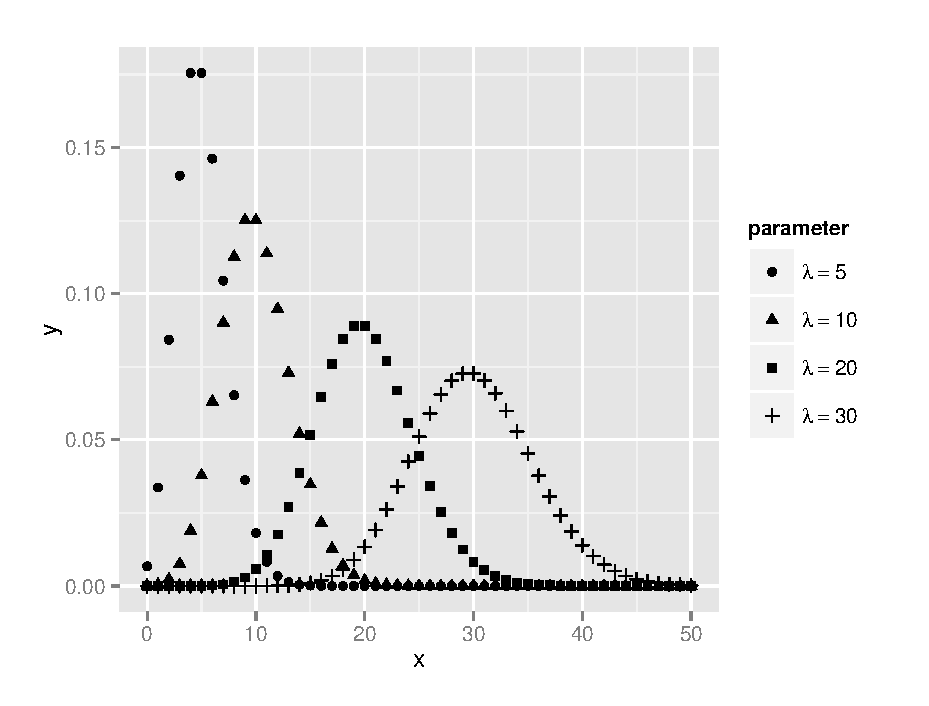
\includegraphics[width=14cm]{Poisson1.eps}
\caption{不同参数下的泊松分布形态}
\label{fig:泊松分布形态}
\end{figure}

从图\ref{fig:泊松分布形态}中可以看出,当$\lambda$的值较大时,泊松分布的概率密度函数形状与正态分布的形状接近,可以考虑用正态分布来近似估计泊松分布的值。为了使近似的效果最好,我们应该保证近似前后的均值和方差不变。$Po(\lambda)$的均值为$\lambda$,方差为$\lambda$,因此如果用正态分布来近似的话,对应的正态分布为$N(\lambda,\lambda)$。

图\ref{fig:泊松分布和正态分布的比较}展示了4个不同参数($\lambda=5,10,20,30$)下,泊松分布$Po(\lambda)$和正态分布$N(\lambda,\lambda)$之间的关系。图中的点是泊松分布$Po(\lambda)$的概率分布,曲线是正态分布$N(\lambda,\lambda)$的概率密度函数。

\begin{figure}[htb]
\centering
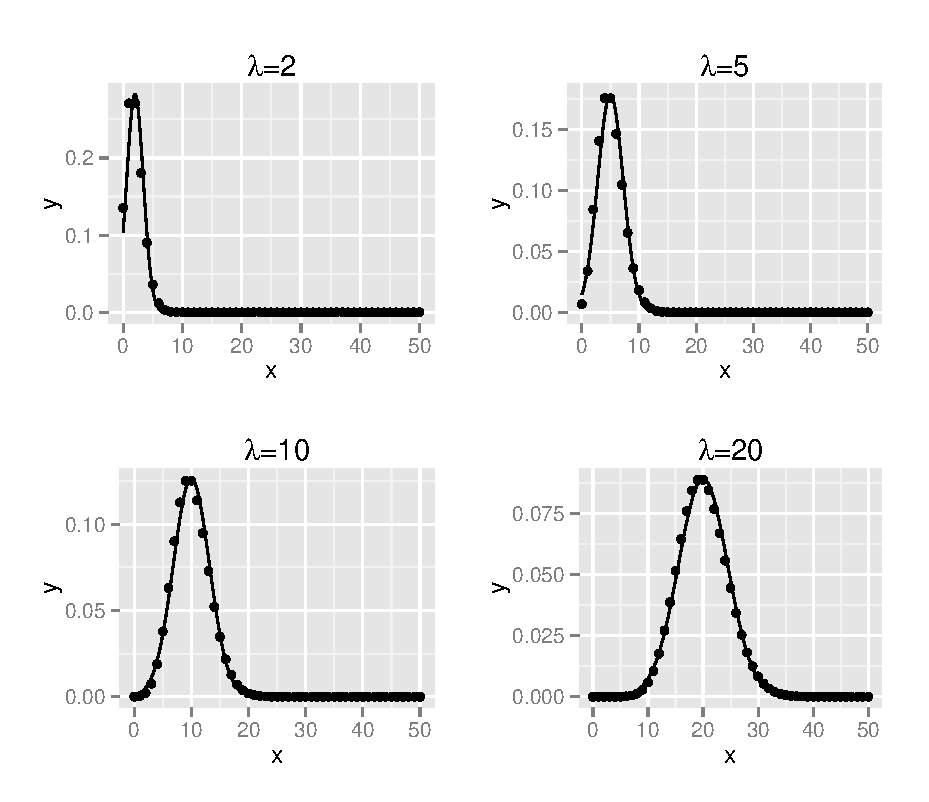
\includegraphics[width=15cm]{Pois_and_Norm.eps}
\caption{$Po(\lambda)$和$N(\lambda,\lambda)$的比较}
\label{fig:泊松分布和正态分布的比较}
\end{figure}

图\ref{fig:泊松分布和正态分布的比较}显示,用正态分布来近似表示泊松分布的效果是比较好的。假设企业的服务水平为$\eta$,对应的正态分布分位数为$z_\eta$,$N$种颜色的成品需求$D_i$服从两两相互独立的泊松分布$Po(\lambda_i)$,需要的库存为$\xi_i$,$i=1,2,\ldots,N$。利用正态分布近似,我们可以计算各成品的库存$\xi_i$的近似值$\hat{\xi_i}$为
\begin{equation}
\hat{\xi_i} = \lambda_i + z_\eta\sqrt{\lambda_i},\qquad i=1,2,\ldots,N
\label{eq:正态近似下的成品库存}
\end{equation}

前面已经证明,两两相互独立的泊松分布之和仍然是泊松分布。若我们取消成品库存,保留在制品库存,则在制品库存的总需求服从泊松分布$Po(\sum_{i=1}^N\lambda_i)$,可近似为正态分布$N(\sum_{i=1}^N\lambda_i,\sum_{i=1}^N\lambda_i)$。需要的在制品库存$\xi$的近似值$\hat{\xi}$为
\begin{equation}
\hat{\xi} = \sum_{i=1}^N\lambda_i + z_\eta\sqrt{\sum_{i=1}^N\lambda_i}
\label{eq:正态近似下的在制品库存}
\end{equation}

根据公式\ref{eq:正态近似下的成品库存}和\ref{eq:正态近似下的在制品库存},可以比较改进前后的库存变化
\begin{align}
\sum_{i=1}^N\hat{\xi_i} - \hat{\xi} &= \sum_{i=1}^N\left(\lambda_i + z_\eta\sqrt{\lambda_i}\right) - \left(\sum_{i=1}^N\lambda_i + z_\eta\sqrt{\sum_{i=1}^N\lambda_i}\right) \notag\\
&= z_\eta\left(\sum_{i=1}^N\sqrt{\lambda_i}-\sqrt{\sum_{i=1}^N\lambda_i}\right) \notag\\
&> z_\eta\left(\sum_{i=1}^N\sqrt{\lambda_i}-\sqrt{\sum_{i=1}^N\lambda_i+2\sum_{i=1}^{N-1}\sum_{j=i+1}^N\sqrt{\lambda_i\lambda_j}}\right) \notag\\
&= z_\eta\left(\sum_{i=1}^N\sqrt{\lambda_i}-\sqrt{\left(\sum_{i=1}^N\sqrt{\lambda_i}\right)^2}\right) \notag\\
&=0
\label{eq:改进前后库存比较_正态近似}
\end{align}

公式\ref{eq:改进前后库存比较_正态近似}证明了,正态近似下,$\hat{\xi} < \sum_{i=1}^N\hat{\xi_i}$是严格成立的。也就是说,改进后的在制品库存小于改进前的各颜色成品库存之和。




\subsection{正态近似的适用性}

我们已经通过正态近似证明,各颜色的成品需求服从相互独立的泊松分布时,通过取消成品库存,保留在制品库存,能够减少企业的总库存。接下来我们将讨论正态近似的适用性。

图\ref{fig:正态近似的误差}展示了4个不同服务水平($\eta=0.75,0.9,0.95,0.99$)下,$\hat{\xi}-\xi$的值随参数$\lambda$的变化。

\begin{figure}[htb]
\centering
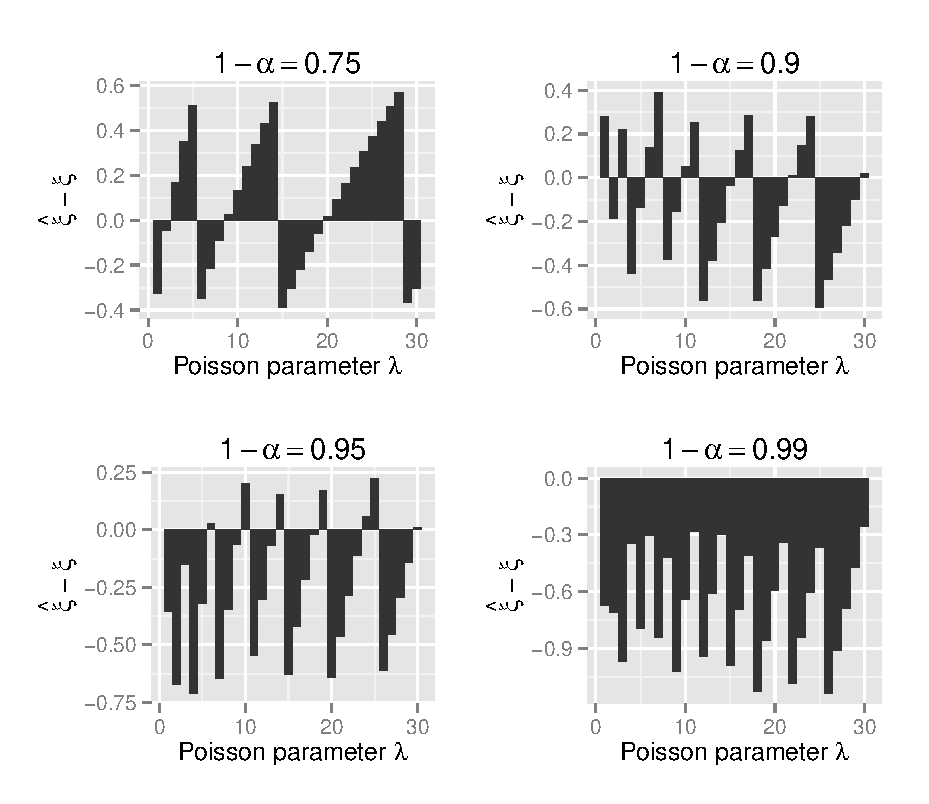
\includegraphics[width=15cm]{Norm_minus_Poisson.eps}
\caption{不同服务水平下正态近似的误差}
\label{fig:正态近似的误差}
\end{figure}

图\ref{fig:正态近似的误差}显示,服务水平越高,正态近似的值越倾向于比真实值小。

我们考虑服务水平为0.99的情况,如图\ref{fig:正态近似的误差}右下所示。此时,对任意的$\lambda$,都有$\hat{\xi} < \xi$;并且对于大多数的$\lambda$,都有$|\hat{\xi} - \xi| < 1$。

若对于任意$i$,都有$|\hat{\xi_i}-\xi_i| < 1$,则$\lceil\hat{\xi_i}\rceil=\xi_i$,结合公式\ref{eq:改进前后库存比较_正态近似}可得
\begin{equation}
\sum_{i=0}^N \xi_i = \sum_{i=0}^N \left\lceil\hat{\xi_i}\right\rceil \geq \left\lceil\sum_{i=0}^N\hat{\xi_i}\right\rceil \geq \left\lceil\hat{\xi}\right\rceil = \xi
\end{equation}

若存在至少一个i,使得$|\hat{\xi_i}-\xi_i| > 1$,则必有$\sum\xi_i \geq \sum\lceil\hat{\xi_i}\rceil + 1$。此时
\begin{equation}
\sum_{i=0}^N \xi_i \geq \sum_{i=0}^N\left\lceil\hat{\xi_i}\right\rceil + 1 \geq \left\lceil\sum_{i=0}^N\hat{\xi_i}\right\rceil + 1 \geq \left\lceil\hat{\xi}\right\rceil + 1 \geq \xi
\end{equation}

因此,对于服务水平为0.99的情况,我们在正态近似下得出的结论是相当可靠的。

当服务水平进一步提高时,$|\hat{\xi_i}-\xi_i|$会继续增大,近似时产生的误差增大,就需要用其他的数值模拟手段来检验改进效果了。

当服务水平降低时,近似的误差开始正向移动。到$\eta=0.75$左右,已经出现大量$\hat{\xi_i} > \xi_i$的情况。此时已不能保证$\sum\xi_i \geq \sum\lceil\hat{\xi_i}\rceil$,上面的放缩方式就不再适用。值得注意的是,$|\hat{\xi_i}-\xi_i|$的值始终是很小的,误差保持在1以内。实际的生产过程是以整数件为单位的,在很多计算环节里都会用到取整,计算过程中增加或减少一件是很正常的事情。因此,1件以内的误差对整个系统的绩效影响不是很大。况且,在这么低的服务水平下,库存应该不是首要考虑目标。

总之,在一般企业的服务水平范围内,正态近似得出的结论基本是可以接受的。






